\documentclass[10pt,letter]{article}
\usepackage{amsmath}
\usepackage{amssymb}
\usepackage{graphicx}
\usepackage{setspace}
%\onehalfspacing
\usepackage{fullpage}
\begin{document}

\title{Problem Set 1}
\author{CS 7641}
\date{Submit by Feb 20, 2014}
\maketitle

Instructions: This problem set is not a part of your final grade. Solve atleast 3 of these problems and submit your solutions on t-square. We will not grade them, but we will provide solutions at the end of the deadline for you to compare your answers. If your final score falls very close to the switchover point to the next higher grade, we will grade your submission of this problem set for input into determining your final grade.

\paragraph{1} 

For almost every case we have discussed where we are doing supervised learning, we have assumed a deterministic function. Imagine instead a world where we are trying to capture a non-deterministic function. In this case, we might see training pairs where the x value appears several times, but with different y values. For example, we might be mapping attributes of humans to whether they are likely to have had chicken pox. In that case, we might see the same “kind” of person many times but sometimes they will have had chicken pox, sometimes not.

We would like to build a learning algorithm that will compute the probability that a particular kind of person has chicken pox. So, given a set of training data where each x is mapped to 1 for true or 0 for false:

\begin{enumerate}
	\item Derive the proper error function to use for finding the ML hypothesis using Bayes Rule. You should go through a similar process as the one used to derive least squared error in the lessons.

	\item Compare and contrast your result to the rule we derived for a deterministic function perturbed by zero-mean gaussian noise. What would a normal neural network using sum of squared errors do with these data?  What if the data consisted of x,y pairs where y was an estimate of the probability instead of 0s and 1s?
\end{enumerate}

\paragraph{2} Design a two-input perceptron that implements the boolean function $A \land \lnot B$. Design a two-layer network of perceptrons that implements $A \oplus B$ ($\oplus$ is XOR).

\paragraph{2 - Answer} Below is a diagram of an XOR ANN:

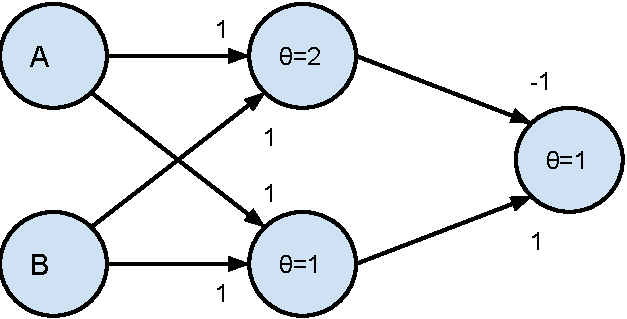
\includegraphics[width=3in]{xor_ann.pdf}

\paragraph{3} Derive the perceptron training rule and gradient descent training rule for a single unit with output $o$, where $o = w_0 + w_1x_1 + w_1x_1^2 + … + w_nx_n + w_nx_n^2$. What are the advantages of using gradient descent training rule for training neural networks over the perceptron training rule?


\paragraph{4} Explain how you can use Decision Trees to perform regression? Show that when the error function is squared error, then the expected value at any leaf is the mean. Take the Boston Housing dataset (https://archive.ics.uci.edu/ml/datasets/Housing) and use Decision Trees to perform regression. 

\paragraph{5} Suggest a lazy version of the eager decision tree learning algorithm ID3. What are the advantages and disadvantages of your lazy algorithm compared to the original eager algorithm?

\paragraph{6} Imagine you had a learning problem with an instance space of points on the plane and a target function that you knew took the form of a line on the plane where all points on one side of the line are positive and all those on the other are negative. If you were constrained to only use decision tree or nearest-neighbor learning, which would you use? Why?

\paragraph{7} Give the VC dimension of the following hypothesis spaces. Briefly explain your answers.
\begin{enumerate}
  \item An origin-centered circle (2D)
  \item An origin-centered sphere (3D)
\end{enumerate}


\end{document}
